\toclesssection{Divide and Conquer}

\toclesssubsection{Concept}

%-------------------------------------------------------------------------------

\begin{frame}{Divide and Conquer}{Introduction}
  \textbf{Concept:}
  \begin{itemize}
    \item<2->
      {\color{MainA}Divide} the problem into smaller subproblems
    \item<3->
      {\color{MainA}Conquer} the subproblems through recursive solving.\\
      If subproblems are small enough solve them directly
    \item<4->
      {\color{MainA}Connect} all subsolutions to solve the overall problem
    \item<5->
      {\color{MainA}Recursive} application of the algorithm on smaller
      subproblems
    \item<6->
      {\color{MainA}Direct} solving of small subproblems
  \end{itemize}
\end{frame}

%-------------------------------------------------------------------------------

\subsection{Maximum Subtotal}

\begin{frame}{Divide and Conquer}{Maximum Subtotal}
  \textbf{Input:}
  \begin{itemize}
    \item<2->
      Sequence {\color{MainA}$X$} of {\color{MainA}$n$} integers
  \end{itemize}
  \textbf{Output:}
  \begin{itemize}
    \item<3->
      Maximum sum of an uninterrupted subsequence of
      {\color{MainA}$X$} and its index boundary
  \end{itemize}
  \vspace{-1em}
  \onslide<4->
  \begin{table}[!t]
    \caption{Input values}
    \begin{tabular}{c|c|c|c|c|c|c|c|c|c|c}
      Index & 0 & 1 & 2 & 3 & 4 & 5 & 6 & 7 & 8 & 9\\
      \midrule
      Value & 31 & -41 & 59 & 26 & -53 & 58 & 97 & -93 & -23 & 84
    \end{tabular}
    \label{tab:divide_and_conquer:max_subtotal_example_values}
  \end{table}
  \vspace{1em}
  %TODO: Hand-Drawings here (Free space) or no free space?
  \textbf{Output:} Sum: 187, Start: 2, End: 6
\end{frame}

%-------------------------------------------------------------------------------

%% \begin{frame}{Divide and Conquer}{Maximum Subtotal}
%%   \begin{example}[Maximum Subtotal]
%%     \vspace{-1em}
%%     \begin{table}[!t]
%%       \caption{Input values}
%%       \begin{tabular}{c|c|c|c|c|c|c|c|c|c|c}
%%         Index & 0 & 1 & 2 & 3 & 4 & 5 & 6 & 7 & 8 & 9\\
%%         \midrule
%%         Value & 31 & -41 & 59 & 26 & -53 & 58 & 97 & -93 & -23 & 84
%%       \end{tabular}
%%       \label{tab:divide_and_conquer:max_subtotal_example_values}
%%     \end{table}
%%     \vspace{6em}
%%     %TODO: Hand-Drawings here (Free space) or no free space?
%%     \textbf{Output:} Sum: 187, Start: 2, End: 6
%%   \end{example}
%% \end{frame}

%-------------------------------------------------------------------------------

\begin{frame}{Divide and Conquer}{Maximum Subtotal}
  \textbf{Idea:}
  \begin{figure}
    \begin{adjustbox}{width=\linewidth}
      \begin{tikzpicture}[
  list/.style={
    draw=black
  }, sum/.style={
    list,
    fill=Hell-Gruen
  }, label_sum/.style={
    color=black,
    font=\huge
  }
]%
% upper list
\draw[list] (0, 0) rectangle ++(16, 1);

\draw[sum] (1.5, 0) rectangle ++(2, 1);
\draw[sum] (13, 0) rectangle ++(2.5, 1);

\node[label_sum, anchor=south] at (2.5, 0) {A};
\node[label_sum, anchor=south] at (14.25, 0) {B};


\draw[list] (8, 1.5) -- (8, -0.5);
\end{tikzpicture}

    \end{adjustbox}
    \label{fig:divide_and_conquer:max_sub_total_divide}
  \end{figure}
  \vspace{-1.5em}
  \begin{itemize}
    \item<2->
      Solve the left / right half of the problem {\color{MainA}recursive}
    \item<3->
      Combine both solutions into a overall solution
    \item<4->
      The maximum is located in the {\color{MainA}left~half~($A$)}
      or the {\color{MainA}right~half~($B$)}
    \item<5->
      The maximum interval can {\color{MainA} overlap with the border ($C$)}
  \end{itemize}
\end{frame}

%-------------------------------------------------------------------------------

\begin{frame}{Divide and Conquer}{Maximum Subtotal}
  \textbf{Principle:}
  \begin{figure}[!h]
    \begin{adjustbox}{width=\linewidth}
      \begin{tikzpicture}[
  list/.style={
    draw=black
  }, sum/.style={
    list,
    fill=Hell-Gruen
  }, label_sum/.style={
    color=black,
    font=\huge
  }
]%
% upper list
\draw[list] (0, 0) rectangle ++(16, 1);

\draw[sum] (1.5, 0) rectangle ++(2, 1);
\draw[sum] (6, 0) rectangle ++(5, 1);
\draw[sum] (13, 0) rectangle ++(2.5, 1);

\node[label_sum, anchor=south] at (2.5, 0) {A};
\node[label_sum, anchor=south] at (14.25, 0) {B};
\node[label_sum, anchor=south] at (7, 0) {rmax};
\node[label_sum, anchor=south] at (9.5, 0) {lmax};

\draw[list] (8, 1.5) -- (8, -0.5);

\draw[
  decorate,
  decoration={brace, raise=0.25em, amplitude=0.5em},
  thick
] (6, 1) -- node[midway, yshift=2em, label_sum] {C} (11, 1);
\end{tikzpicture}
    \end{adjustbox}
    \label{fig:divide_and_conquer:max_sub_total_divide2}
  \end{figure}
  \vspace{-1.5em}
  \begin{itemize}
    \item<2->
      Small problems are solved directly:
      {\color{MainA}$n = 1 \Rightarrow \max = X[0]$}
    \item<3->
      Big problems are decomposed into two subproblems and solved recursively.
      Subsolutions {\color{MainA}$A$} and {\color{MainA}$B$}
      are returned
    \item<4->
      To solve {\color{MainA}$C$} we have to calculate
      {\color{MainA}rmax} and {\color{MainA}lmax}
    \item<5->
      Overall solution is maximum of {\color{MainA}$A$}
      {\color{MainA}$B$} and {\color{MainA}$C$}
  \end{itemize}
\end{frame}

%-------------------------------------------------------------------------------

\codeslide{python}{
\begin{frame}{Divide and Conquer}{Maximum Subtotal - Python}
  \vspace{-0.5em}
  \lstinputlisting[
    language=Python,
    basicstyle=\small,
    tabsize=4,
    style={python-idle-code},
    escapechar={@},
    emph={maxSubArray,lmax,rmax},
    emphstyle=\color{blue},
    breaklines=false
  ]{Code/DivideAndConquer/MaxSubTotal_DivideAndConquer.py}
\end{frame}

%-------------------------------------------------------------------------------

\begin{frame}{Divide and Conquer}{Maximum Subtotal - Python}
  \vspace{-0.5em}
  \lstinputlisting[
    language=Python,
    basicstyle=\small,
    tabsize=4,
    style={python-idle-code},
    escapechar={@},
    emph={maxSubArray},
    emphstyle=\color{blue}
  ]{Code/DivideAndConquer/MaxSubTotal_SecondTrivialCase.py}
\end{frame}

%-------------------------------------------------------------------------------

\begin{frame}{Divide and Conquer}{Maximum Subtotal - Python}
  \vspace{-0.5em}
  \lstinputlisting[
    language=Python,
    basicstyle=\small,
    tabsize=4,
    style={python-idle-code},
    escapechar={@},
    emph={maxSubArray},
    emphstyle=\color{blue}
  ]{Code/DivideAndConquer/MaxSubTotal_Max.py}
\end{frame}

%-------------------------------------------------------------------------------

\begin{frame}{Divide and Conquer}{Maximum Subtotal - Python}
  \vspace{-0.5em}
  \lstinputlisting[
    language=Python,
    basicstyle=\small,
    tabsize=4,
    style={python-idle-code},
    escapechar={@},
    emph={maxSubArray},
    emphstyle=\color{blue}
  ]{Code/DivideAndConquer/MaxSubTotal_Max2.py}
\end{frame}
%-------------------------------------------------------------------------------

\begin{frame}{Divide and Conquer}{Maximum Subtotal - Python}
  \vspace{-0.5em}
  \lstinputlisting[
    language=Python,
    basicstyle=\small,
    tabsize=4,
    style={python-idle-code},
    escapechar={@},
    emph={lmax},
    emphstyle=\color{blue}
  ]{Code/DivideAndConquer/MaxSubTotal_LMax.py}
\end{frame}

%-------------------------------------------------------------------------------

\begin{frame}{Divide and Conquer}{Maximum Subtotal - Python}
  \vspace{-0.5em}
  \lstinputlisting[
    language=Python,
    basicstyle=\small,
    tabsize=4,
    style={python-idle-code},
    escapechar={@},
    emph={rmax},
    emphstyle=\color{blue}
  ]{Code/DivideAndConquer/MaxSubTotal_RMax.py}
\end{frame}
}

%TODO: Implement for Java / C++

%-------------------------------------------------------------------------------

\begin{frame}{Divide and Conquer}{Maximum Subtotal}
  \begin{table}
    \caption{\textit{lmax} example}
    \label{fig:divide_and_conquer:lmax_example}
    \begin{tabular}{c|cccccc}
      index & $i$ & $i+1$ & $\cdots$ & $\cdots$ & $j-1$ & $j$\\
      %\midrule
      $X$ & 58 & -53 & 26 & 59 & -41 & 31\\
      %\midrule
       {\color{MainA}$sum$} & 58 & 5 & 31 & 90 & 49 & 80\\
      {\color{MainA}$lmax$} & 58 & 58 & 58 & 90 & 90 & 90\\
    \end{tabular}
  \end{table}
  \begin{itemize}
    \item<2->
      The {\color{MainA}$sum$} and {\color{MainA}$lmax$} are initialized with $X[i]$
    \item<3->
      We iterate over {\color{MainA}$X$} from {\color{MainA}$i+1$} to {\color{MainA}$j$} and update {\color{MainA}$sum$}
    \item<4->
      If {\color{MainA}$sum > lmax$} then {\color{MainA}$lmax$}
      gets updated
  \end{itemize}
\end{frame}

%-------------------------------------------------------------------------------

\begin{frame}{Divide and Conquer}{Maximum Subtotal}
  \begin{tabular}{l}
\onslide<1>{\rlap{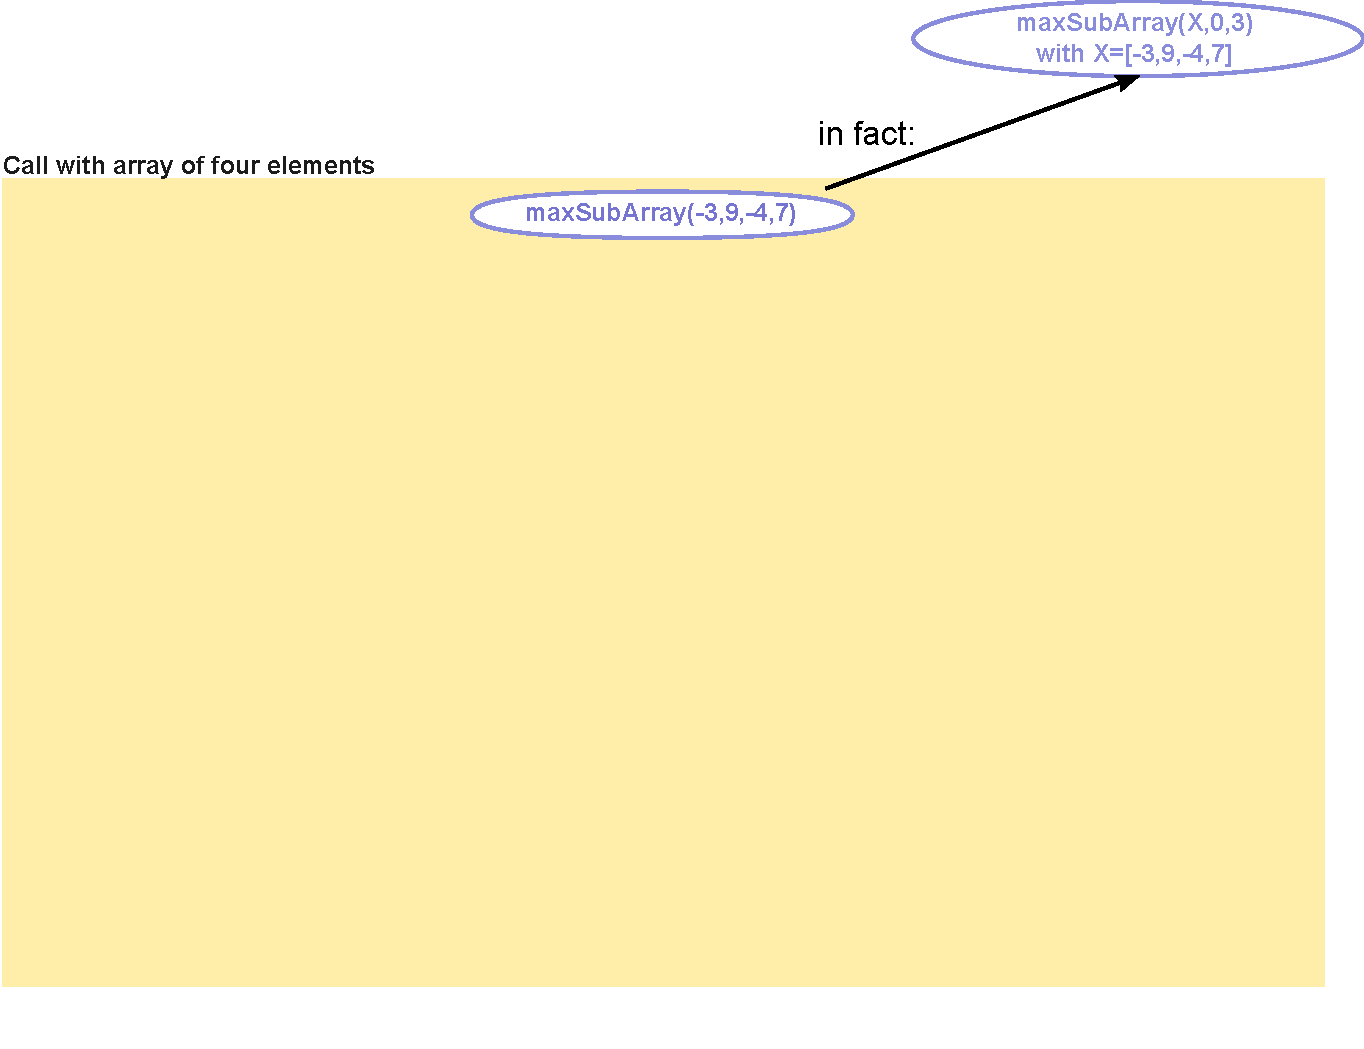
\includegraphics[width=1\textwidth]{Images/DivideAndConquer/maxsubarray-o1.pdf}}}%
\onslide<2>{\rlap{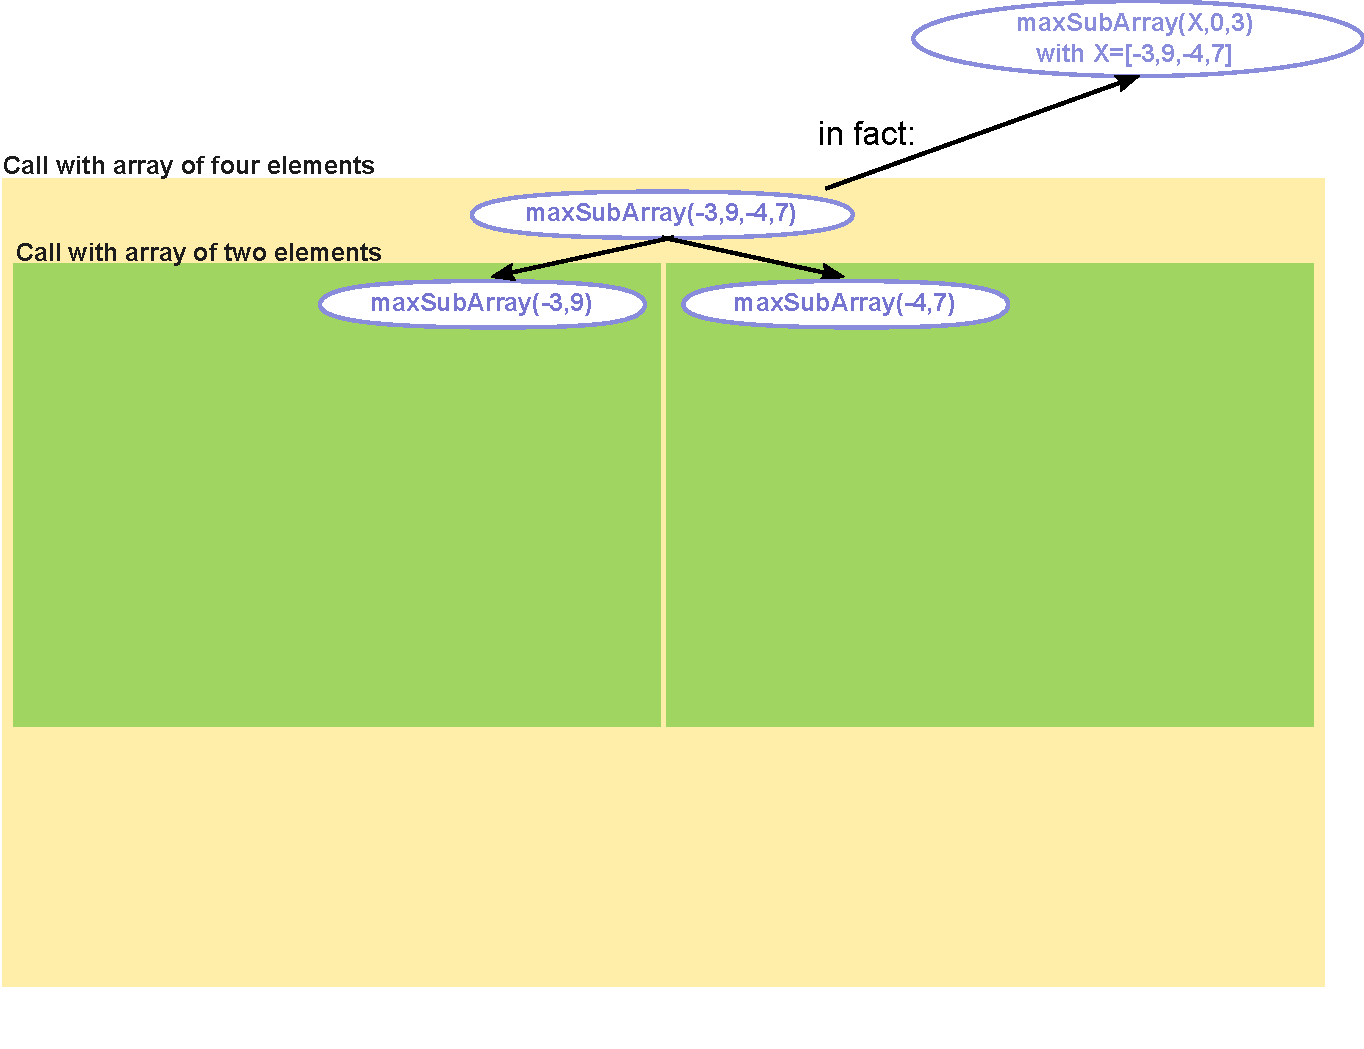
\includegraphics[width=1\textwidth]{Images/DivideAndConquer/maxsubarray-o2.pdf}}}%
\onslide<3>{\rlap{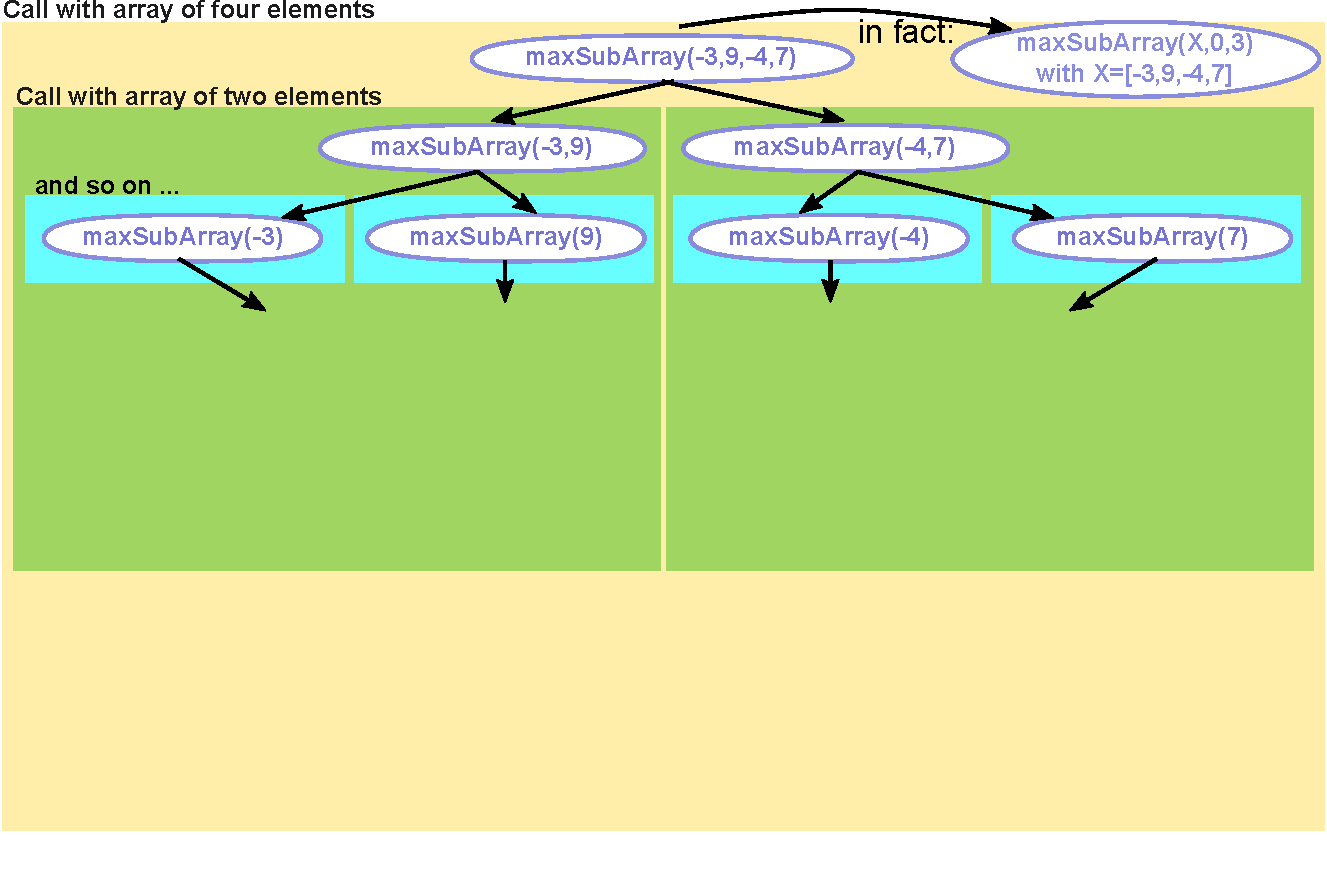
\includegraphics[width=1\textwidth]{Images/DivideAndConquer/maxsubarray-o3.pdf}}}%
\onslide<4>{\rlap{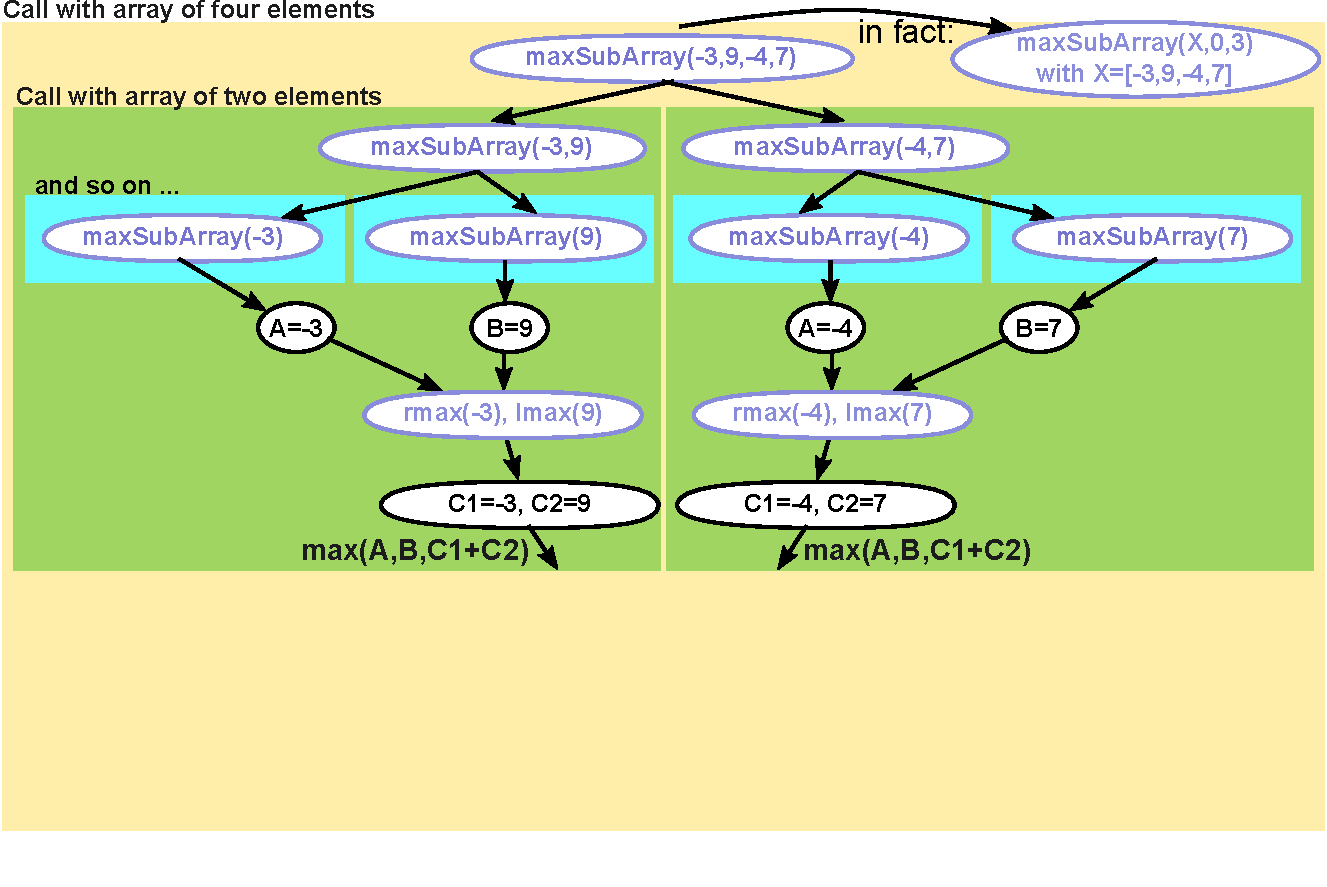
\includegraphics[width=1\textwidth]{Images/DivideAndConquer/maxsubarray-o4.pdf}}}%
\onslide<5->{\rlap{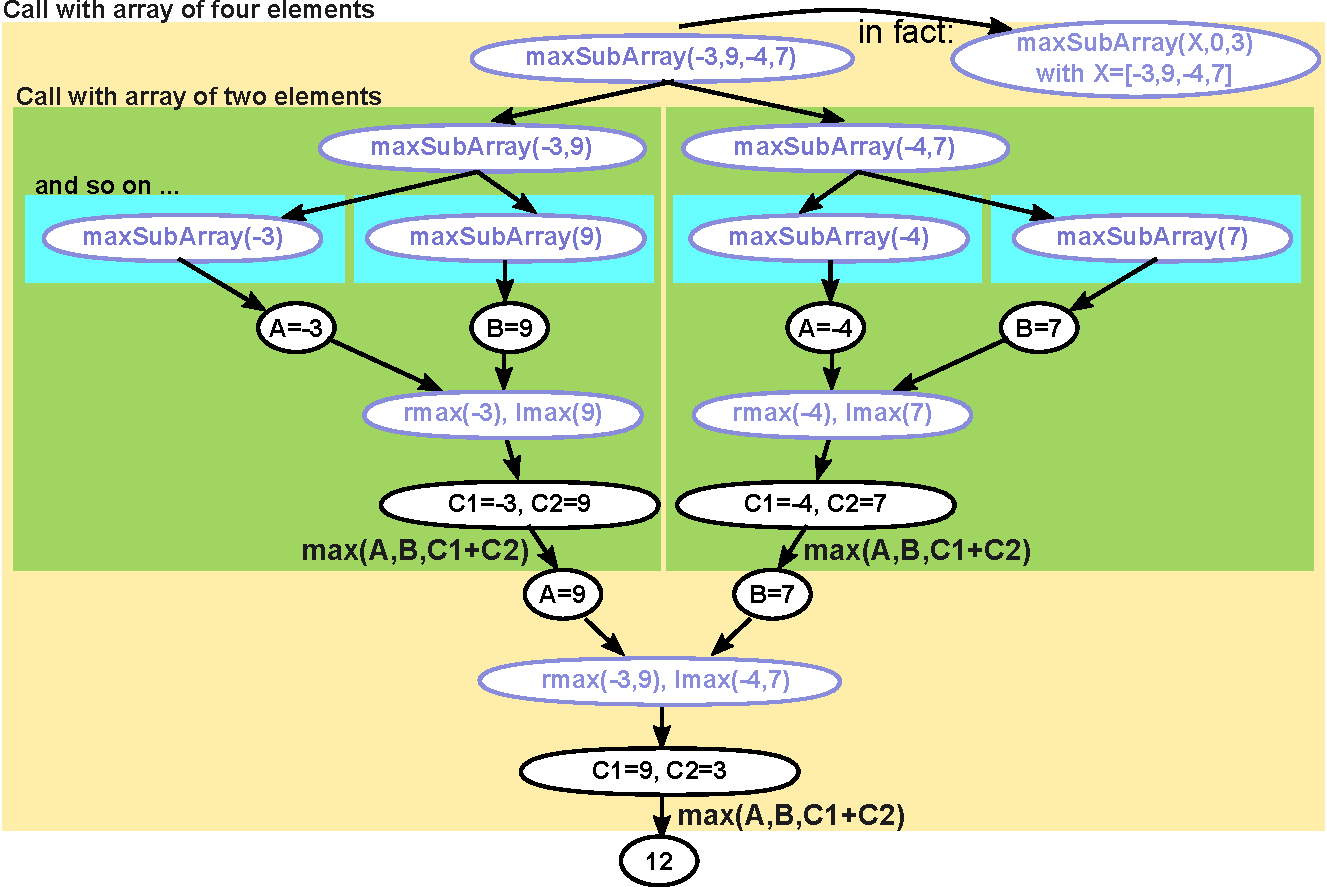
\includegraphics[width=1\textwidth]{Images/DivideAndConquer/maxsubarray-o5.pdf}}}%
  \end{tabular}
\end{frame}

%-------------------------------------------------------------------------------

% \begin{frame}{Divide and Conquer}{Maximum Subtotal}
%   \begin{figure}
%     \begin{adjustbox}{width=\linewidth}
%       \begin{tikzpicture}[
  op/.style={
   draw=black,
   color=black,
   fill=white,
   thick,
   ellipse
  }, sum/.style={
    draw,
    rectangle,
    text=Mittel-Gruen
  }, max/.style={
    text=Mittel-Gruen
  }, array_label/.style={
    color=Mittel-Blau,
    fill=white
  }, arrow/.style={
    ultra thick,
    color=Mittel-Gruen
  }
]%
% Main Problem with first-level subproblems
\only<1-2>{
  \node[op, label={[array_label]below:$X[0:4]=[-3,9,-4,7]$}]
    (root) at (0, 0) {\textit{maxSubArray}(X, 0, 3)};

  \node[op, anchor=east, label={[array_label]below:$X[0:2]=[-3,9]$}]
    (left) at (-0.25, -2) {\textit{maxSubArray}(X, 0, 1)};
  \node[op, anchor=west, label={[array_label]below:$X[2:4]=[-4,7]$}]
    (right) at (0.25, -2) {\textit{maxSubArray}(X, 2, 3)};
}

% Second-level subproblems
\only<2->{
  \node[op, anchor=east, label={[array_label]below:$X[0:1]=[-3]$}]
    (left_triv_left) at (-4.5, -4) {\textit{maxSA}(X, 0, 0)};
  \node[op, anchor=east, label={[array_label]below:$X[1:2]=[9]$}]
    (left_triv_right) at (-0.25, -4) {\textit{maxSA}(X, 1, 1)};

  \node[op, anchor=west, label={[array_label]below:$X[2:3]=[-4]$}]
    (right_triv_left) at (0.25, -4) {\textit{maxSA}(X, 2, 2)};
  \node[op, anchor=west, label={[array_label]below:$X[3:4]=[7]$}]
    (right_triv_right) at (4.5, -4) {\textit{maxSA}(X, 3, 3)};
}

% Combination of second-level solutions
\only<4->{
  \node[max] at (-8, -7.0) {$max$};
}
% Dummy nodes for slides < display
\only<3>{ % Dummy node
  \node[color=white] (sum_left) at (-4, -7.0) {$A=-3, B=9, C=lmax+rmax=6$};
}
\only<3-4>{ % Dummy node
  \node[color=white] (sum_right) at (4, -7.0) {$A=-4, B=7, C=lmax+rmax=3$};
}

\only<4->{
  \node[sum] (sum_left) at (-4, -7.0) {$A=-3, B=9, C=lmax+rmax=6$};
}
\only<5->{
  \node[sum] (sum_right) at (4, -7.0) {$A=-4, B=7, C=lmax+rmax=3$};
}

\only<4->{
  \node[max] at (-8, -7.0) {$max$};
}
% Dummy nodes for slides < display
\only<3>{ % Dummy node
  \node[color=white] (sum_left) at (-4, -7.0) {$A=-3, B=9, C=lmax+rmax=6$};
}

% Combination of second-level solutions
\only<7->{
  \node[max] at (-8, -9) {$max$};
}
% Dummy nodes for slides < display
\only<3-6>{ % Dummy node
  \node[color=white] (sum) at (0, -9) {$A=9, B=7, C=lmax+rmax=12$};
}
\only<7->{
  \node[sum] (sum) at (0, -9) {$A=9, B=7, C=lmax+rmax=12$};
  \node[max] (sum_total) at (0, -10) {$12$};
}

\only<3->{ % Results of second-level problems
  \node[array_label, anchor=east, xshift=1.5em]
    at ($(sum_left)!0.35!(left_triv_left)$) {$A=-3, rmax=-3$};
  \node[array_label, anchor=west, xshift=-1.5em]
    at ($(sum_left)!0.35!(left_triv_right)$) {$B=9, lmax=9$};

  \node[array_label, anchor=east, xshift=1.5em]
    at ($(sum_right)!0.35!(right_triv_left)$) {$A=-4, rmax=-4$};
  \node[array_label, anchor=west, xshift=-1.5em]
    at ($(sum_right)!0.35!(right_triv_right)$) {$B=7, lmax=7$};
}
\only<6->{ % Results of first-level problems
  \node[array_label]
    at ($(sum.north west)!0.4!(sum_left)$) {$A=9, rmax=9$};
  \node[array_label]
    at ($(sum.north east)!0.4!(sum_right)$) {$B=7, lmax=3$};
}

\begin{pgfonlayer}{background}
  % Draw the arrows for the first split
  \only<1-2>{
    \draw[->, arrow] (root) -- (left);
    \draw[->, arrow] (root) -- (right);
  }
  % Draw the arrows for the second split
  \only<2>{
    \draw[->, arrow] (left) -- (left_triv_left);
    \draw[->, arrow] (left) -- (left_triv_right);
    \draw[->, arrow] (right) -- (right_triv_left);
    \draw[->, arrow] (right) -- (right_triv_right);
  }
  % Draw the arrows for the second-level solutions
  \only<3->{
    \draw[->, arrow] (left_triv_left) -- (sum_left);
    \draw[->, arrow] (left_triv_right) -- (sum_left);
    \draw[->, arrow] (right_triv_left) -- (sum_right);
    \draw[->, arrow] (right_triv_right) -- (sum_right);
  }
  % Draw the arrows for the first-level solutions
  \only<6->{
    \draw[->, arrow] (sum_left) -- (sum.north west);
    \draw[->, arrow] (sum_right) -- (sum.north east);
  }
  \only<7>{
    \draw[->, arrow] (sum) -- (sum_total);
  }
\end{pgfonlayer}
\end{tikzpicture}
%     \end{adjustbox}
%     \caption{\textit{maxSubArray} with $X = [-3, 9, -4, 7]$}
%     \label{fig:divide_and_conquer:max_sub_array_example}
%   \end{figure}
% \end{frame}

%-------------------------------------------------------------------------------

\codeslide{python}{
\begin{frame}{Divide and Conquer}{Maximum Subtotal - Python}
  \vspace{-0.5em}
  \lstinputlisting[
    language=Python,
    basicstyle=\small,
    tabsize=4,
    style={python-idle-code},
    breaklines=false,
    escapechar={@},
    emph={maxSubArray,lmax,rmax},
    emphstyle=\color{blue}
  ]{Code/DivideAndConquer/MaxSubTotal_Runtime.py}
\end{frame}
}

%TODO: Implement for Java / C++

%-------------------------------------------------------------------------------

\begin{frame}{Divide and Conquer}{Maximum Subtotal - Number of steps $T(n)$}
  \textbf{Recursion equation:} 
  \begin{displaymath}
    T(n) = \begin{cases}
      \hfill \underbrace{\Theta(1)}_\text{trivial case} & n = 1\\
      \underbrace{2 \cdot T\left(\frac{n}{2}\right)}_\text{
        solving of subproblems
      } + \underbrace{
        \Theta(n)
        \vphantom{\left(\frac{n}{2}\right)}
      }_\text{combination of solutions} & n > 1
    \end{cases}
  \end{displaymath}
    \begin{itemize}
    \item<2->
      There exist two constants {\color{MainA}$a$} and {\color{MainA}$b$} with:
      \begin{displaymath}
        T(n) \leq \begin{cases}
          \hfill {\color{MainA}a} & n = 1\\
          2 \cdot T\left(\frac{n}{2}\right) + {\color{MainA}b} \cdot n & n > 1
        \end{cases}
      \end{displaymath}
    \item<3->
      We define {\color{MainA}$c := \max(a,b)$}:
      \begin{displaymath}
        T(n) \leq \begin{cases}
          \hfill {\color{MainA}c} & n = 1\\
          2 \cdot T\left(\frac{n}{2}\right) + {\color{MainA}c} \cdot n & n > 1
        \end{cases}
      \end{displaymath}
  \end{itemize}
\end{frame}

%-------------------------------------------------------------------------------

%% \begin{frame}{Divide and Conquer}{Maximum Subtotal - Number of steps $T(n)$}
%%   \begin{itemize}
%%     \item
%%       There exist two constants $a$ and $b$ with:
%%       \begin{displaymath}
%%         T(n) \leq \begin{cases}
%%           \hfill a & n = 1\\
%%           2 \cdot T\left(\frac{n}{2}\right) + b \cdot n & n > 1
%%         \end{cases}
%%       \end{displaymath}
%%     \item
%%       We define $c := \max(a,b)$:
%%       \begin{displaymath}
%%         T(n) \leq \begin{cases}
%%           \hfill c & n = 1\\
%%           2 \cdot T\left(\frac{n}{2}\right) + c \cdot n & n > 1
%%         \end{cases}
%%       \end{displaymath}
%%   \end{itemize}
%% \end{frame}

%-------------------------------------------------------------------------------

\begin{frame}{Divide and Conquer}{Maximum Subtotal - Illustration of $T(n)$}
  \begin{figure}
    \begin{adjustbox}{width=\linewidth}
      \begin{tikzpicture}[
  op/.style={
    draw=black,
    fill=white,
    font=\Large,
    thick,
    ellipse,
    minimum height=3em
  }, sum/.style={
    font=\Large,
    text=Mittel-Blau
  }, connection/.style={
    ultra thick,
    color=Mittel-Gruen
  }, arrow/.style={
    ultra thick,
    color=Mittel-Blau
  }, arrow_alt/.style={
    ultra thick,
    color=Hell-Blau
  }, label/.style={
    font=\Large,
    text=Mittel-Blau
  }, label_alt/.style={
    font=\Large,
    text=Hell-Blau
  }
]%
% Bounding boxes
\only<1>{\draw[white] (-8, -4) rectangle (8, 4);}
\only<2>{\draw[white] (-8, -5) rectangle (8, 3);}
\only<3->{\draw[white] (-8, -6) rectangle (8, 2);}

% Main Problem with first-level subproblems
\node[op] (root) at (0, 0) {%
  \only<1>{$T(n)$}%
  \only<2->{$c \cdot n$}%
};

\only<2-5>{
  \node[op] (left) at (-1.5, -2) {%
    \only<2>{$T\left(\frac{n}{2}\right)$}%
    \only<3->{$c \cdot \frac{n}{2}$}%
  };
  \node[op] (right) at (1.5, -2) {%
    \only<2>{$T\left(\frac{n}{2}\right)$}%
    \only<3->{$c \cdot \frac{n}{2}$}%
  };
  
  \draw[-, connection] (root) -- (left);
  \draw[-, connection] (root) -- (right);
}
\only<2>{
  \node[sum] at (0, -3.5) {%
    $T(n) = 2 \cdot T\left(\frac{n}{2}\right) + c \cdot n$%
  };
}

\only<3-5>{
  \node[op] (left_left) at (-4.0, -4) {$T\left(\frac{n}{4}\right)$};
  \node[op] (left_right) at (-1.5, -4) {$T\left(\frac{n}{4}\right)$};
  \node[op] (right_left) at (1.5, -4) {$T\left(\frac{n}{4}\right)$};
  \node[op] (right_right) at (4.0, -4) {$T\left(\frac{n}{4}\right)$};
  
  \draw[-, connection] (left) -- (left_left);
  \draw[-, connection] (left) -- (left_right);
  \draw[-, connection] (right) -- (right_left);
  \draw[-, connection] (right) -- (right_right);
  
  \node[sum] at (-2.75, -5.5) {%
    \begin{math}%
      T\left(\frac{n}{2}\right)
      = 2 \cdot T\left(\frac{n}{4}\right) + c \cdot \frac{n}{2}
%      \Rightarrow
%      T(n) = 4 \cdot T\left(\frac{n}{4}\right)
%        + c \cdot \left(n + \frac{n}{2}\right)
    \end{math}%
  };
}

\begin{pgfonlayer}{background}
\only<4>{
  \node[label, anchor=north west] (comb) at (-7, 1) {combining solutions};
  
  \draw[->, arrow] (comb.south) -- (root);
  \draw[->, arrow] (comb.south) -- (left);
  \draw[->, arrow] (comb.south) -- (right);
}
\only<5>{
  \node[label, anchor=north east] (solv) at (7, 1) {solving subproblems};
  
  \draw[->, arrow] (solv.south) -- (left_left);
  \draw[->, arrow] (solv.south) -- (left_right);
  \draw[->, arrow] (solv.south) -- (right_left);
  \draw[->, arrow] (solv.south) -- (right_right);
}
\end{pgfonlayer}
\end{tikzpicture}
    \end{adjustbox}
    \caption{Illustration of the runtime}
    \label{fig:divide_and_conquer:max_sub_array_runtime}
  \end{figure}
\end{frame}

%-------------------------------------------------------------------------------

\begin{frame}{Divide and Conquer}{Maximum Subtotal - Illustration of $T(n)$}
  \begin{figure}
    \begin{adjustbox}{width=\linewidth}
      \begin{tikzpicture}[
  op/.style={
    draw=black,
    fill=white,
    font=\Large,
    thick,
    ellipse,
    minimum size=3em
  }, sum/.style={
    font=\Large,
    text=Mittel-Blau
  }, connection/.style={
    ultra thick,
    color=Mittel-Gruen
  }, arrow/.style={
    ultra thick,
    color=Mittel-Blau
  }, label/.style={
    fill=white,
    font=\Large,
    text=black
  }
]%
% Bounding boxes
\draw[white] (-10, -9) rectangle (9.5, 1);

% Main Problem with first-level subproblems
\node[op] (root) at (-4, 0) {$c \cdot n$};
\node[sum, anchor=west, align=left] at (2, 0) {%
  {\color{Mittel-Blau}1} node processing
  {\color{Mittel-Blau}$n$} elements\\
  \hspace{1.5em}{\color{Mittel-Blau}%
    \begin{math}
      \Rightarrow c \cdot n
    \end{math}%
  }
};

\only<2->{
  \node[op] (left) at (-5.5, -2) {$c \cdot \frac{n}{2}$};
  \node[op] (right) at (-2.5, -2) {$c \cdot \frac{n}{2}$};
  
  \draw[-, connection] (root) -- (left);
  \draw[-, connection] (root) -- (right);
  
  \node[sum, anchor=west, align=left] at (2, -2) {%
    {\color{Mittel-Blau}2} nodes processing
    {\color{Mittel-Blau}$\frac{n}{2}$} elements\\
    \hspace{1.5em}{\color{Mittel-Blau}%
      \begin{math}
        \Rightarrow 2 \, c \cdot \frac{n}{2}
          = c \cdot n
      \end{math}%
    }
  };
}

\only<3->{
  \node[op] (left_left) at (-7.0, -4) {$c \cdot \frac{n}{4}$};
  \node[op] (left_right) at (-5.0, -4) {$c \cdot \frac{n}{4}$};
  \node[op] (right_left) at (-3.0, -4) {$c \cdot \frac{n}{4}$};
  \node[op] (right_right) at (-1.0, -4) {$c \cdot \frac{n}{4}$};
  
  \draw[-, connection] (left) -- (left_left);
  \draw[-, connection] (left) -- (left_right);
  \draw[-, connection] (right) -- (right_left);
  \draw[-, connection] (right) -- (right_right);
  
  \node[sum, anchor=west, align=left] at (2, -4) {%
    {\color{Mittel-Blau}4} nodes processing
    {\color{Mittel-Blau}$\frac{n}{4}$} elements\\
    \hspace{1.5em}{\color{Mittel-Blau}%
      \begin{math}
        \Rightarrow 4 \, c \cdot \frac{n}{4}
          = c \cdot n
      \end{math}%
    }
  };
}

\only<4->{
  \node[op] (left_left_left) at (-8.375, -6) {$\cdots$};
  \node[op] (left_left_right) at (-7.125, -6) {$\cdots$};
  \node[op] (left_right_left) at (-5.875, -6) {$\cdots$};
  \node[op] (left_right_right) at (-4.625, -6) {$\cdots$};
  \node[op] (right_left_left) at (-3.375, -6) {$\cdots$};
  \node[op] (right_left_right) at (-2.125, -6) {$\cdots$};
  \node[op] (right_right_left) at (-0.875, -6) {$\cdots$};
  \node[op] (right_right_right) at (0.375, -6) {$\cdots$};
  
  \draw[-, connection] (left_left) -- (left_left_left);
  \draw[-, connection] (left_left) -- (left_left_right);
  \draw[-, connection] (left_right) -- (left_right_left);
  \draw[-, connection] (left_right) -- (left_right_right);
  \draw[-, connection] (right_left) -- (right_left_left);
  \draw[-, connection] (right_left) -- (right_left_right);
  \draw[-, connection] (right_right) -- (right_right_left);
  \draw[-, connection] (right_right) -- (right_right_right);
  
  \node[sum, anchor=west, align=left] at (2, -6) {%
    {\color{Mittel-Blau}$2^i$} nodes processing
    {\color{Mittel-Blau}$\frac{n}{2^i}$} elements\\
    \hspace{1.5em}{\color{Mittel-Blau}%
      \begin{math}
      \Rightarrow 2^i \, c \cdot \frac{n}{2^i}
      = c \cdot n
      \end{math}%
    }
  };
}

\only<5->{
  \node[op] (left_left_left_c) at (-8.375, -8) {$c$};
  \node[op] (left_left_right_c) at (-7.125, -8) {$c$};
  \node[op] (left_right_left_c) at (-5.875, -8) {$c$};
  \node[op] (left_right_right_c) at (-4.625, -8) {$c$};
  
  \node[op] (right_left_left_c) at (-3.375, -8) {$c$};
  \node[op] (right_left_right_c) at (-2.125, -8) {$c$};
  \node[op] (right_right_left_c) at (-0.875, -8) {$c$};
  \node[op] (right_right_right_c) at (0.375, -8) {$c$};
  
  \draw[-, connection] (left_left_left) -- (left_left_left_c);
  \draw[-, connection] (left_left_right) -- (left_left_right_c);
  \draw[-, connection] (left_right_left) -- (left_right_left_c);
  \draw[-, connection] (left_right_right) -- (left_right_right_c);
  
  \draw[-, connection] (right_left_left) -- (right_left_left_c);
  \draw[-, connection] (right_left_right) -- (right_left_right_c);
  \draw[-, connection] (right_right_left) -- (right_right_left_c);
  \draw[-, connection] (right_right_right) -- (right_right_right_c);
  
  \node[sum, anchor=west, align=left] at (2, -8) {%
    {\color{Mittel-Blau}$n$} nodes processing
    {\color{Mittel-Blau}$1$} element\\
    \hspace{1.5em}{\color{Mittel-Blau}$\Rightarrow c \cdot n$}
  };
  
  \draw[<->, arrow] (-9.5, 0.5)
    to node[label, pos=0.25, anchor=west, align=left, xshift=-1.25em] {%
      {\color{Mittel-Blau}$\log_2n + 1$}\\%
      layers%
    } (-9.5, -8.5);
}
\end{tikzpicture}
    \end{adjustbox}
    \caption{Recursion tree method}
    \label{fig:divide_and_conquer:max_sub_array_runtime_tree}
  \end{figure}
\end{frame}

%-------------------------------------------------------------------------------

\begin{frame}{Divide and Conquer}{Maximum Subtotal - Illustration of $T(n)$}
  \textbf{Depth:}
  \begin{itemize}
    \item<2->
      Top level with depth {\color{MainA}$i = 0$}
    \item<3->
      Lowest level with {\color{MainA}$2^i = n$} elements
      \begin{displaymath}
        {\color{MainA}\Rightarrow i = \log_2 n}
      \end{displaymath}
  \end{itemize}
  \onslide<4->
  \textbf{Runtime:}
  \begin{itemize}
    \item<5->
      A total of {\color{MainA}$\log_2 n + 1$} levels with each cost of
      {\color{MainA}$c \cdot n$}\\
      \color{gray}
      The costs of merging the solutions and solving of the trivial
      problems are the same here
  \end{itemize}
  \onslide<6->
  \begin{displaymath}
    {\color{MainA}
    T(n) = c \cdot n \log_2 n + c \cdot n \in \Theta(n\,\log n)}
  \end{displaymath}
\end{frame}

%-------------------------------------------------------------------------------

\begin{frame}{Divide and Conquer}{Maximum Subtotal - Summary}
  \textbf{Summary:}
  \begin{itemize}
    \item<2->
      Direct solution is slow with {\color{MainA}$\mathcal{O}(n^3)$}
    \item<3->
      Better solution with incremental update of sum was
      {\color{MainA}$\mathcal{O}(n^2)$}
    \item<4->
      Divide and conquer approach results in
      {\color{MainA}$\mathcal{O}(n\,\log n)$}
    \item<5->
      There is an approach running in {\color{MainA}$\mathcal{O}(n)$}
      if you assume that all subtotals are positive
  \end{itemize}
\end{frame}

%-------------------------------------------------------------------------------

\begin{frame}{Divide and Conquer}{Maximum Subtotal}
  \begin{figure}
    \begin{adjustbox}{width=\linewidth}
      \begin{tikzpicture}[
  list/.style={
    draw=black
  }, sum/.style={
    list,
    fill=Hell-Gruen
  }, label_sum/.style={
    color=black,
    font=\huge
  }
]%
% upper list
\draw[list] (0, 0) rectangle ++(18, 1);

\draw[sum] (1.5, 0) rectangle ++(3, 1);
\draw[sum] (7, 0) rectangle ++(5, 1);

\node[label_sum, anchor=south] at (3, 0) {\texttt{tMax}};
\node[label_sum, anchor=south] at (9.5, 0) {\texttt{rMax}};

\node[label_sum, anchor=south] at (12, 1.5) {\texttt{i}};
\node[label_sum, anchor=south, align=center] (text)
  at (7, 2) {point of last\\negative subtotal};

\draw[->, color=Mittel-Blau, line width=0.25em] (text.south) -- (7, 1.0);

\draw[list, dashed] (12, 1.5) -- (12, -0.5);
\end{tikzpicture}
    \end{adjustbox}
    \caption{Scanning the array in linear time}
    \label{fig:divide_and_conquer:max_sub_total_linear}
  \end{figure}
\end{frame}

\codeslide{python}{
\begin{frame}{Divide and Conquer}{Maximum Subtotal - Python}
  \vspace{-0.5em}
  \lstinputlisting[
    language=Python,
    basicstyle=\small,
    tabsize=4,
    style={python-idle-code},
    breaklines=false,
    escapechar={@},
    emph={maxSubArray},
    emphstyle=\color{blue}
  ]{Code/DivideAndConquer/MaxSubTotal_LinearRuntime.py}
\end{frame}
}

%TODO: Implement for Java / C++
